\section{Theorie}
\label{sec:Theorie}
In der Geometrischen Optik wird von Lichtstrahlen ausgegangen, die sich geradlinig im Raum ausbreiten.
Diese Lichtstrahlen können an einem optisch dichteren Medium gebrochen werden.
Bei dem Übergang in ein Anderes Medium wird ein Teil der Lichtstrahlen reflektiert und ein Teil erfährt eine
Richtungsänderung.
Als Medium werden Linsen betrachtet, dabei wird zwischen Sammellinsen und Zerstreuungslinsen
differenziert.
Eine dünne Sammellinse ist in Abbildung \ref{fig:duenn} d.argestellt
\begin{figure}
 \centering
 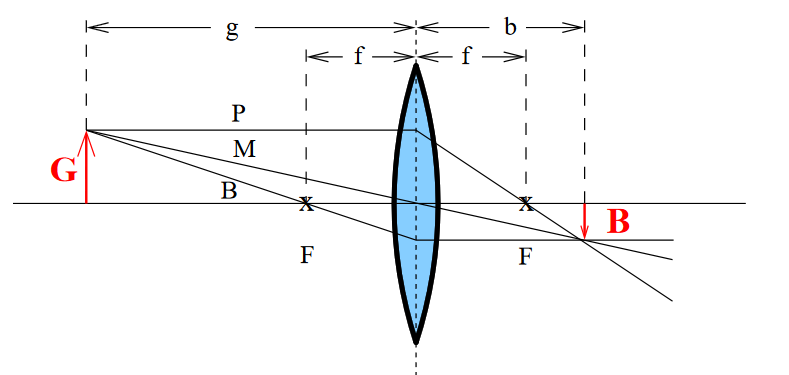
\includegraphics[width=0.5\textwidth]{duenn.png}
 \caption{Darstellung einer dünnen Linse.\cite{sample}}
 \label{fig:duenn}
 \end{figure}
Die Sammellinse sammelt parallele Lichtstrahlen in dem Brennpunkt $F$. Die Brennweite $f$ und die Bildweite $b$
sind positiv, somit entsteht ein reelles Bild. Im Gegensatz dazu sind die beiden Größen bei einer Zerstreuungslinse,
zu sehen in Abbildung \ref{fig:streu}, negativ und es kommt zu einem virtuellem Bild.
\begin{figure}
 \centering
 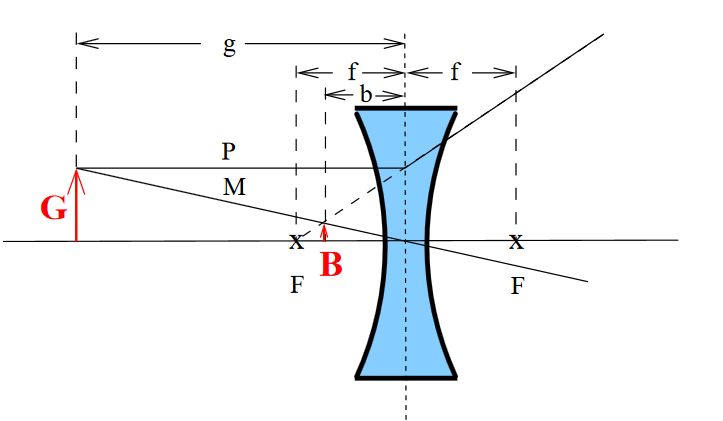
\includegraphics[width=0.5\textwidth]{streu.png}
 \caption{Darstellung einer Zerstreuungslinse.\cite{sample}}
 \label{fig:streu}
 \end{figure}

Zur geometrischen Beschreibung dienen drei Strahlen die vom Gegenstand ausgehen:
\begin{itemize}
 \item Mittelpuntsstrahl $M$: verläuft durch den Mittelpunkt der Linse ohne Richtungsänderung.
 \item Parallelstrahl $P$: verläuft bis zur Mittelebene der Linse parallel zur optischen Achse,
       wird danach gebrochen und geht durch den Brennpunkt.
 \item Brennpunktstrahl $B$: verläuft durch den Brennpunkt zur Mittelebene der Linse, wird dort gebrochen und verläuft
       anschließend paralell zur optischen Achse.
\end{itemize}
Aus den Strahlen-Konstruktionen folgt zum einen das Abbildungsgesetz:
\begin{align}
V=\frac{B}{G} = \frac{b}{g}.
\end{align}
Dies besagt, dass sich der Abbildungsmaßstab $V$ von Bildgröße $B$ zur Gegenstandsgröße $G$  verhält wie die
Bildweite $b$ zur Gegenstandsweite $g$.
Für dünne Linsen lässt sich weiterhin die Linsengleichung folgern:
\begin{align}
\frac{1}{f}=\frac{1}{b}+\frac{1}{g}\label{eqn:linse}.
\end{align}
Für dicke Linsen gilt die Brechung an der Mittelebene der Linse nicht mehr, dazu werden zwei Hauptebenen $H$
und $H'$ eingeführt und angenommen, dass die Strahlen an diesen gebrochen werden.
Die Größen $b$, $f$ und $g$ beziehen sich dann auf die jeweilige Hauptebene. Mit dieser Anpassung
behält die Linsengleichung auch bei dicken Linsen ihre Gültigkeit.
Ebenfalls problematisch ist die Brechung an Mittelebene und Hauptebene bei achsfernen Strahlen,
durch eine stärkere Brechung dieser Strahlen kommt es zu Abbildungsfehlern, auch Linsenfehler genannt.
Im Falle der sphärischen Abberation befindet sich der Brennpunkt der achsfernen Strahlen
näher an der Linse als jener der achsnahen.
Wie stark ein Lichtstrahl gebrochen wird hängt auch von der Wellenlänge des Lichts ab, so liegt der Brennpunkt
von blauem Licht näher an der Linse als der vom roten Licht, dieses Phänomen wird chromatische Abberation
genannt.
